%%%%%%%%%%%%%%%%%%%%%%%%%%%%%%%%%%%%%%%%%%%%%%%%%%%%%%%%%%%%%%%%%%%%%%%%%%%%
%%%  NiteOutMag --- At Least the Web Remembers What Happened Last Night  %%%
%%%%%%%%%%%%%%%%%%%%%%%%%%%%%%%%%%%%%%%%%%%%%%%%%%%%%%%%%%%%%%%%%%%%%%%%%%%%

\documentclass{acm_proc_article-sp}

\usepackage[utf8]{inputenc}
\usepackage[T1]{fontenc}
\usepackage[activate=compatibility]{microtype}

% autoref command
\usepackage[pdftex,urlcolor=black,colorlinks=true,linkcolor=black,citecolor=black]{hyperref}
\def\sectionautorefname{Section}
\def\subsectionautorefname{Subsection}
\def\subfloatautorefname{Subfigure}

\usepackage[lofdepth,lotdepth]{subfig}
\usepackage{enumitem}
\usepackage{textcomp}
\usepackage{mathtools}
\usepackage{url}

% give emph a normal fontsize
\let\oldemph\emph
\renewcommand{\emph}[1]{\oldemph{\fontsize{9}{9}\selectfont #1}}

% more readable footnote layout
\renewcommand{\footnotesize}{\fontsize{8pt}{10pt}}
\setlength{\footnotesep}{.5cm}

% todo macro
\usepackage{color}
\newcommand{\todo}[1]{\noindent\textcolor{red}{{\bf \{TODO}: #1{\bf \}}}}

% listings and Verbatim environment
\usepackage{fancyvrb}
\usepackage{relsize}
\usepackage{listings}
\usepackage{verbatim}
\newcommand{\defaultlistingsize}{\fontsize{8pt}{9.5pt}}
\newcommand{\inlinelistingsize}{\fontsize{8pt}{11pt}}
\newcommand{\smalllistingsize}{\fontsize{7.5pt}{9.5pt}}
\newcommand{\listingsize}{\defaultlistingsize}
\RecustomVerbatimCommand{\Verb}{Verb}{fontsize=\inlinelistingsize}
\RecustomVerbatimEnvironment{Verbatim}{Verbatim}{fontsize=\defaultlistingsize}
\lstset{frame=lines,captionpos=b,numberbychapter=false,escapechar=§,
        aboveskip=0.5em,belowskip=0em,abovecaptionskip=0em,belowcaptionskip=0em,
framexbottommargin=-1em,
        basicstyle=\ttfamily\listingsize\selectfont}

\usepackage{color}
\definecolor{lightgray}{rgb}{.9,.9,.9}
\definecolor{darkgray}{rgb}{.4,.4,.4}
\definecolor{purple}{rgb}{0.65, 0.12, 0.82}

\lstdefinelanguage{JavaScript}{
  keywords={typeof, new, true, false, catch, function, return, null, catch, switch, var, if, in, while, do, else, case, break},
  keywordstyle=\color{blue}\bfseries,
  ndkeywords={class, export, boolean, throw, implements, import, this},
  ndkeywordstyle=\color{darkgray}\bfseries,
  identifierstyle=\color{red},
  sensitive=false,
  showstringspaces=false,
  comment=[l]{//},
  morecomment=[s]{/*}{*/},
  commentstyle=\color{purple}\ttfamily,
  stringstyle=\color{gray}\ttfamily,
  morestring=[b]',
  morestring=[b]"
}

% use Courier from this point onward, except for URLs
\let\oldttdefault\ttdefault
\renewcommand{\ttdefault}{pcr}
\let\oldurl\url
\renewcommand{\UrlFont}{\fontfamily{\oldttdefault}\selectfont}

% linewrap symbol
\definecolor{grey}{RGB}{130,130,130}
\newcommand{\linewrap}{\raisebox{-.6ex}{\textcolor{grey}{$\hookleftarrow$}}}

% for 1st, 2nd, etc. superscripting
\newcommand{\ts}{\textsuperscript}

% more pleasing quote environment
\usepackage{tikz}
\newcommand*{\openquote}{\tikz[remember picture,overlay,xshift=-7pt,yshift=1pt]
     \node (OQ) {\fontfamily{fxl}\fontsize{16}{16}\selectfont``};\kern0pt}
\newcommand*{\closequote}{\tikz[remember picture,overlay,xshift=2pt,yshift=-4.5pt]
     \node (CQ) {\fontfamily{fxl}\fontsize{16}{16}\selectfont''};}
\renewenvironment{quote}%
{\setlength{\parindent}{1cm}\par\openquote}
{\closequote\vspace{-4.5pt}
}

%%%%%%%%%%%%%%%%%%%%%%%%%%%%%%%
%%%  Beginning of document  %%%
%%%%%%%%%%%%%%%%%%%%%%%%%%%%%%%

\begin{document}

% --- Author Metadata here ---
%\conferenceinfo{WOODSTOCK}{'97 El Paso, Texas USA}
%\CopyrightYear{2007} % Allows default copyright year (20XX) to be over-ridden - IF NEED BE.
%\crdata{0-12345-67-8/90/01}  % Allows default copyright data (0-89791-88-6/97/05) to be over-ridden - IF NEED BE.
% --- End of Author Metadata ---

\title{NiteOutMag\hspace{-1.5pt}\raisebox{6pt}{$^\textbf{\sffamily TM}$}---At Least the Web\\ Remembers What Happened Last Night}

\numberofauthors{5}
\author{
% Tom, Ruben, Raphaël, Giuseppe, José
}

%\author{
%\alignauthor
%\textbf{Thomas Steiner}\\
%	\affaddr{Univ. Polit\`{e}cnica de Catalunya}\\
%	\affaddr{Department LSI}\\
%	\affaddr{08034 Barcelona, Spain,}\\
%	\affaddr{tsteiner@lsi.upc.edu}
%\alignauthor
%\textbf{Ruben Verborgh}\\ 	
%	\affaddr{Ghent University -- IBBT, ELIS}\\
%	\affaddr{Multimedia Lab}\\
%	\affaddr{9050 Ghent, Belgium}\\
%	\affaddr{ruben.verborgh@ugent.be}	
%\alignauthor
%\textbf{Rapha\"el Troncy}\\
%	\affaddr{EURECOM}\\
%	\affaddr{06560 Sophia Antipolis}\\
%	\affaddr{France}\\
%	\affaddr{raphael.troncy@eurecom.fr}
%\and
%\alignauthor
%\textbf{Jos\'e Luis Redondo Garcia}\\
%	\affaddr{EURECOM}\\
%	\affaddr{06560 Sophia Antipolis}\\
%	\affaddr{France}\\
%	\affaddr{redondo@eurecom.fr}
%\alignauthor
%\textbf{Giuseppe Rizzo}\\
%	\affaddr{EURECOM}\\
%	\affaddr{06560 Sophia Antipolis}\\
%	\affaddr{France}\\
%	\affaddr{rizzo@eurecom.fr}
%}

\maketitle

%%%%%%%%%%%%%%%%%%
%%%  Abstract  %%%
%%%%%%%%%%%%%%%%%%

\begin{abstract}
The chorus of the popular song \emph{TiK ToK} by the artist \emph{Ke\$ha}\footnote{\url{https://www.youtube.com/watch?v=iP6XpLQM2Cs}} goes \emph{``Don't stop, make it pop. DJ, blow my speakers up. Tonight, I'mma fight. 'Til we see the sunlight. Tik tok on the clock. But the party don't stop, no.''}. We all know, however, that each party comes to an end eventually. With NiteOutMag\texttrademark, we present a~Chrome Web application that can help people recover what (the hell) happened last night. Among the younger generation, nightlife activities---just about like any other activity---together with related multimedia data get shared online on social networks. The problem is that for one and the same event, the event-related user-generated data may be shared on a~plethora of social networks. Therefore, for this challenge, we introduce an application that leverages description of events from several event databases, social data from multiple social networks, and media data from some media sharing platforms. The data collected is attached to events held in a given area and further processed to generate an event-centric magazine where each page represents an event illustrated by media. Just like the nightlife of people happens \emph{ad hoc} from one party to the other, the NiteOutMag\texttrademark~application gathers as well all its data on-the-fly, without the burden of pre-compiled data directories. The application is available online at \url{http://goo.gl/fjuE5}. A screencast showcasing the application is also available\footnote{\url{https://t.co/3R8h2RnW}}.
\end{abstract}

%\category{H.3.4}{Information Systems}{Information Storage and Retrieval}[World Wide Web]
%\category{H.3.5}{Online Information Services}{Web-based services}

%\keywords{}

%%%%%%%%%%%%%%%%%%%%%%%%%
%%%  1. Introduction  %%%
%%%%%%%%%%%%%%%%%%%%%%%%%

\section{Introduction}                                                      \label{sec:introduction}
In March 2012, 901 million monthly active users of the social networking site (SNS) Facebook have uploaded more than 300 million photos on average per day~\cite{Facebook2012}. Many of those photos are event-related and typically illustrate events such as music concerts that a user has attended. Facebook, however, albeit the biggest, is only one among a plethora of social networks that people use to share event-related content. In the following, we list the SNSs considered for NiteOutMag\texttrademark.

A social network is an online service or media platform that focuses on building and reflecting social relationships among people sharing interests and/or activities. In this paper, we consider eleven different social networks that represent all together most of the Western world's market share. In detail, the considered social networks are
\mbox{Google+} (\url{google.com/+}),
Myspace (\url{myspace.com}),
Facebook (\url{facebook.com}),
Twitter ({\url{twitter.com}),
Instagram (\url{instagram.com}),
Flickr (\url{flickr.com}),
YouTube (\url{youtube.com}),
yfrog (\url{yfrog.com}),
MobyPicture (\url{mobypicture.com}),
Twitpic (\url{twitpic.com}), and
\mbox{img.ly} (\url{img.ly}).

The actual detection of events based on information from SNSs is out of scope for this paper. We observe that this has become a very active research field. For example, Petkos \emph{et al.} propose to detect events using a multimodal clustering approach~\cite{Petkos2012}. In this paper, we will consider event databases that maintain listings of past and upcoming events using crowd sourcing techniques and that can be queried programmatically. More precisely, we consider four event databases, namely Eventful (\url{eventful.com}), Foursquare \\(\url{foursquare.com}), Upcoming (\url{upcoming.org}), and Google Places (\url{google.com/places}).

In this paper, we propose to generate fully automatically an event-centric magazine where each page correspond to a known event that is illustrated with media shared on the web. The remainder of this paper is organized as follows. Section~\ref{sec:related-work} presents some related work aiming at creating summaries and narratives of events using social media. Section~\ref{sec:implementation} details our approach: we start from a given location and we collect the events and their illustrative media in a recent past before assembling a digital magazine. In Section~\ref{sec:experiments}, we present and discuss the results we obtained on an experiment. Finally, we give our conclusions and outline future work in Section~\ref{sec:conclusion}.

%%%%%%%%%%%%%%%%%%%%%%%%%
%%%  2. Related Work  %%%
%%%%%%%%%%%%%%%%%%%%%%%%%

\section{Related Work}                                                      \label{sec:related-work}
Capturing life moments and building narratives using social networks is addressed in~\cite{Atosy2011}, where the authors investigated about the interaction between event stories and the use of social networks to tell them. They proposed Storify~\cite{Storify2012}, a web application which supports users to perform story telling and in particular: (1) sorting and organizing the items of an experience similar to the elements of a story, (2) communicating and discussing strategies on how to guide a user towards an intended experience. The overall storytelling creation is supervised by the user, who describes the story as a crafted experience~\cite{Hassenzahl2010}. Streams of news navigate through the social platforms such as Twitter, YouTube. Getting the big picture from them is the objective of Storyful~\cite{Storyful2012}. This application allows the user to navigate through the story created by other users or to create his own aggregating the content available from Twitter, Youtube and adding more.

Events have a key role in the human life and illustrating events with media items stemming from social networks is a very active research topic. In~\cite{Brenner2012}, Brenner and Izquierdo present an approach to detect social events and retrieve associated photos in collaboratively annotated photo collections combining data of various modalities such as time, location, and textual and visual features. In~\cite{Liu2011}, Liu \emph{et al.} present a method for combining semantic inferencing and visual analysis for automatically gathering photos and videos illustrating events. Regarding esthetic aspects of media compilation, in~\cite{Sandhaus2011}, Sandhaus \emph{et al.} consider visual and esthetic features for the automatic creation of photo books. Obrador \emph{et al.} use visual and esthetic features for a category-based approach to automatically assess the esthetic appeal of photographs~\cite{Obrador2012}.

%%%%%%%%%%%%%%%%%%%%%%%%%%%
%%%  3. Implementation  %%%
%%%%%%%%%%%%%%%%%%%%%%%%%%%

\section{Implementation}                                                    \label{sec:implementation}
In this section, we provide the implementation details of the NiteOutMag\texttrademark application. It is implemented as a Chrome application since this technique provides a transparent statement about the required resources of the application, \emph{i.e.}, cross-domain access to event databases and search APIs.

\subsection{Geocoding}
The application focuses on events that occurred in a~certain area. While event databases tend to work based on concrete GPS points like
\mbox{(40.7590110, -73.98447220)}, \emph{i.e.}, a pair composed of a latitude and a longitude, human beings use more human-friendly place names such as \emph{Times Square, New York}. Geocoding is the process of finding the geographic coordinates (generally expressed as latitude and longitude) associated to other geographic data such as an address composed of a street name and a zip code. The user can enter an exact address, such as \emph{618 W. 46th St, New York, NY 10036}, or a~very broad area like \emph{Las Vegas}. The returned latitude and longitude pair is always the center of the particular area of interest. In our implementation, we use the Google Geocoding API~\cite{Geocoding2012}.

\subsection{Event Search}
Based on a latitude and longitude pair, we search for events that took place near this location (in a radius of five kilometers) in a recent past using the respective event search APIs~\cite{Eventful2012,Foursquare2012,GooglePlaces2012,Upcoming2012}. We sanitize the event titles by removing HTML tags, punctuation,
common abbreviations (such as \emph{w/}, which becomes \emph{with}, or \emph{ft./feat.}, which becomes \emph{featuring}). Event directories can overlap in their coverage. Therefore, we deduplicate the returned set of events based on the simple, yet effective Levenshtein distance on the event titles with an empirically determined editing distance of five. Hence, we are capable to find that the event names \emph{Titanic} and \emph{Titanic 3D} correspond to the same movie event.

\subsection{Media Search} \label{sec:media-search}
Unlike event search, media search in our application is \emph{not} based on geolocation. According to a study performed in May 2012 by Seline~\cite{Quora2012},
only roughly 1\% of all microposts on Twitter are geotagged. In addition to that, as our approach covers more SNSs than Twitter, we need to consider that not all SNSs support geotagging of content. In consequence, we use a two-tier approach for media search. Let's illustrate this by a real event of a Beach Boys concert\footnote{\url{http://www.thebeachboys.com/\#tour}} in the Merriweather Post Pavilion in Columbia, MD. The event name is \emph{Beach Boys},
the venue name is \emph{Merriweather Post Pavilion}, and the area is \emph{Columbia, Maryland (MD)}. We define as \emph{human-friendly address} the first part up to the comma of the \texttt{formatted\_address} field in the Google Geocoding API~\cite{Geocoding2012}, \emph{i.e.}, \emph{Columbia} in this case. Human beings aware of the local context do not need to disambiguate, \emph{i.e.}, there is no need to explicitly state \emph{MD}. The two-tier approach consists thus of a full-text search for:
\begin{itemize}
 \item \emph{(i)} the (event name) $+$ the (venue name), and
 \item \emph{(ii)} the (event name) $+$ the (human-friendly address).
\end{itemize}

We have implemented a media collector consisting of media extractors for all SNSs listed in \autoref{sec:introduction}.
% DOUBLE-BLIND REVIEW
% This media collector was first described in~\cite{Khrouf2012}.
% DOUBLE-BLIND REVIEW
It takes a search term as input, \emph{e.g.}, \emph{Beach Boys Columbia} for the example above, and then performs a parallel full-text search using the search APIs of all SNSs. When all the media extractors have responded, a unified SNS-agnostic output is delivered. We propose a common alignment schema, illustrated in
\autoref{lst:media}, which shows the resulting metadata for an exemplary media item. The \autoref{fig:architecture} depicts the overall architecture of the media collector.

\begin{lstlisting}[language=JavaScript,caption={Sample output of the media collector showing a~\mbox{Google+} post (edited for legibility, URLs shortened).},label={lst:media}]
{
  "mediaurl": "http://t.co/ubagkiR9",
  "storyurl": "https://t.co/dau5pBWD",
  "message": {
    "text": "My wife, who once said her vision of
        heaven was being on the lawn bouncing
        around beach balls at a Beach Boys
        concert [...]
        <a href=\"http://t.co/pH2OV1fW\" >
        http://t.co/pH2OV1fW</a> [...]",
    "clean": "My wife, who once said her vision of
        heaven was being on the lawn bouncing
        around beach balls at a Beach Boys
        concert [...]"
  },
  "user": "https://t.co/gIf2UVZR",
  "type": "photo",
  "timestamp": 1329342797000,
  "published": "2012-02-15T21:53:17.000Z"
}
\end{lstlisting}

\begin{figure*}[htb!]
\centering
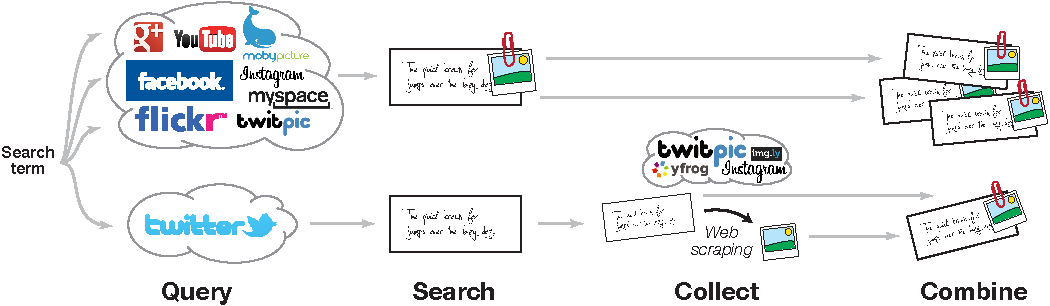
\includegraphics[width=0.8\linewidth]{./architecture.pdf}
\caption{Overview of the media collector: hybrid approach for the media item extraction process using a~combination of API access and Web scraping}
\label{fig:architecture}
\end{figure*}

\subsection{Magazine Layout}
In order to create the illusion of a~real magazine,
flipping from page to page needs to be as credible as possible.
The open-source library turn.js by Emmanuel García~\cite{TurnJs2012}
allows for the dynamic creation of magazines solely based on HTML5 technologies
with a~very realistic page flip effect.
We treat each event as one page of the magazine,
add the event metadata as headline and subheading of the page,
and arrange the images and accompanying microposts to fill the page.
For each event, we use the image with the highest resolution
as background image of the page in order to create a~lifestyle magazine appearance.
For additional print-like look and feel, we use drop caps,
as can be seen in \autoref{fig:screenshot}.
The title page gets dynamically created based on a~Google image search
for the (human-friendly address) $+$ the keyword (nightlife).

\subsection{Installation Instructions}
The NiteOutMag\texttrademark application requires the Chrome browser.
Download the application from the URL \url{http://goo.gl/fjuE5} to the local file system.
Once there, drag and drop it into the \url{chrome://chrome/extensions/} page in the browser.
When you drop it on the extensions page, you will notice an install option popping up there.
When you agree to install, you will see the standard installation dialog
that informs you about the rights that the application is requesting.
It needs access to the before-mentioned event databases and media search APIs.

%%%%%%%%%%%%%%%%%%%%%%%%
%%%  4. Experiments  %%%
%%%%%%%%%%%%%%%%%%%%%%%%

\section{Experiments}                                                       \label{sec:experiments}
We have evaluated our application with the top ten list of
United States cities by
population\footnote{\url{http://en.wikipedia.org/wiki/List_of_United_States_cities_by_population}}
with promising results.

\begin{figure}[b!]
\centering
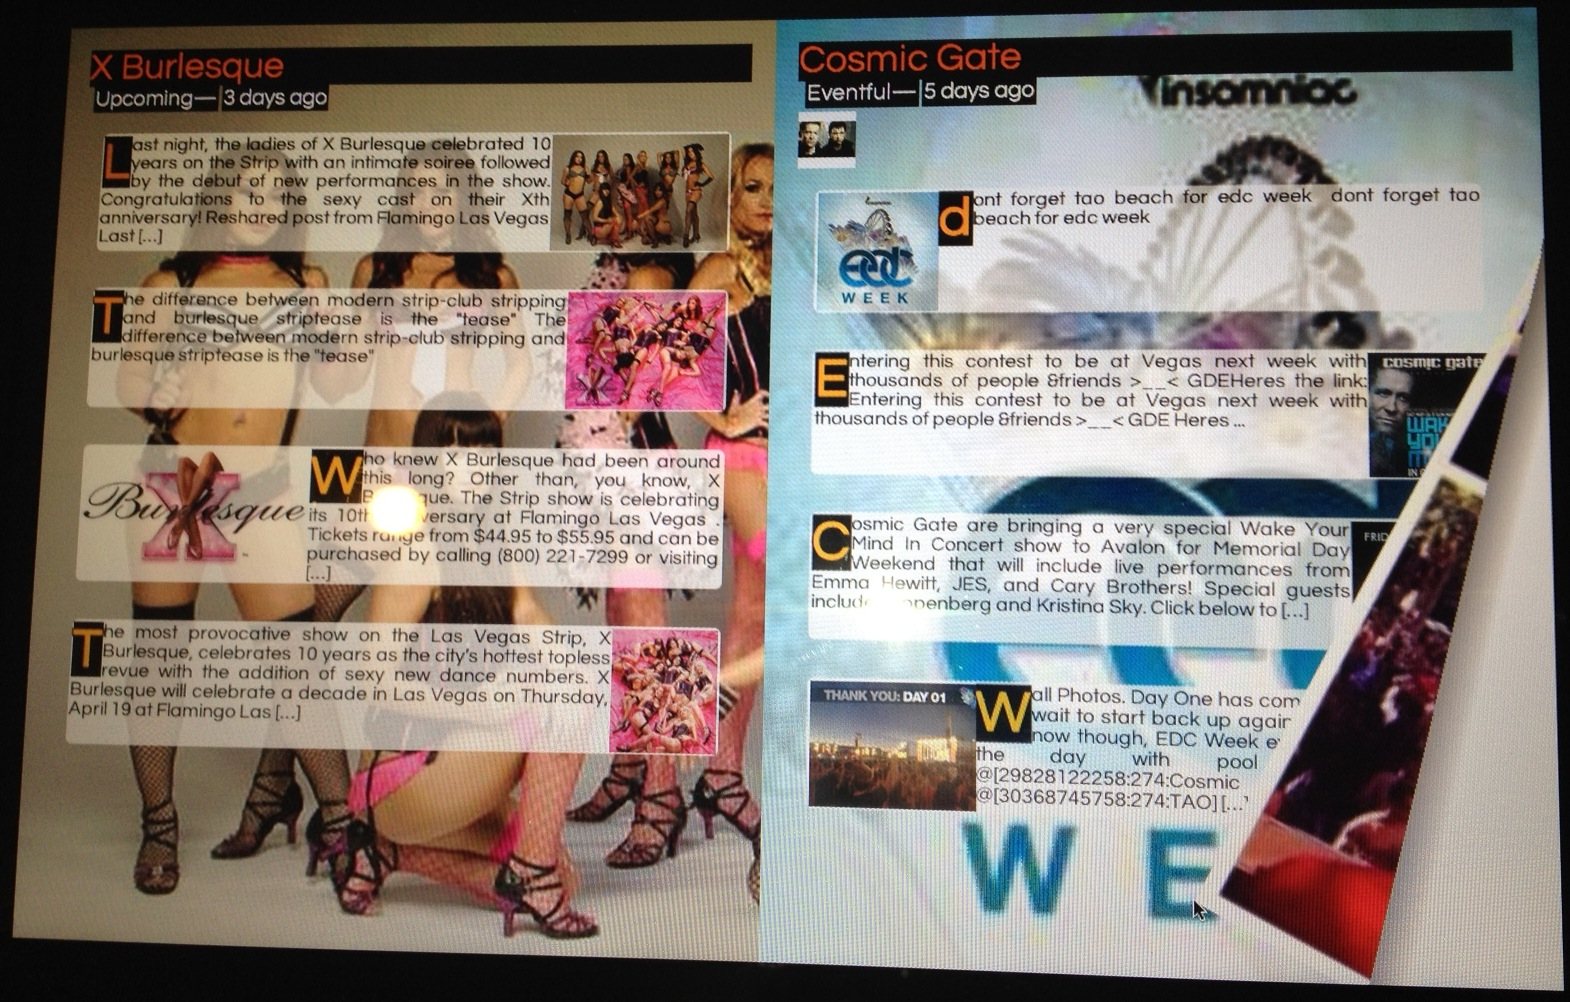
\includegraphics[width=1.0\columnwidth]{./screenshot.jpg}
\caption{Screenshot of the NiteOutMag\texttrademark application with two events from Las Vegas and the righthand-side page about to be flipped}
\label{fig:screenshot}
\end{figure}

\subsection{Query Examples}
In general, big cities and well-known places of interest
reveal good results due to the high density of events.
Popular examples are among others
(\emph{Fisherman's Wharf, San Francisco}),
(\emph{Times Square, New York}),
(\emph{Piccadilly Circus, London}),
or simply (\emph{Ibiza}).	
A~manually compiled list of America's top party cities
from the magazine Maxim\footnote{\url{http://www.maxim.com/movies/americas-top-10-party-cities}}
also reveals interesting results.

\subsection{Discussion and Future Work}
The results stand and fall with the quality of the events
in the event databases.
One problem are stuffed event titles like
\emph{Kandyland 2012 @ the Playboy Mansion -- 1.877.VIP.MANS\-ION}\footnote{\url{http://t.co/YUm7FtmE}},
where the actual event title gets combined with the venue name
and a~vanity contact phone number.
Detection of such stuffed titles is difficult and needs more work.

Event deduplication is a~second issue.
The two movie events \emph{The Avengers} and
\emph{Marvel's The Avengers 3D} are the same for a~human being,
however, for a~machine, the duplication is harder to detect.
Media item deduplication is a~task that we have left for future work.

The system's response time is improvable.
The main issue here is the browser-enforced maximum number
of simultaneous HTTP requests.
With our current four event sources that we have limited
to ten events per source, we already have up to forty events
that we need to search media items for.
As outlined before in \autoref{sec:media-search},
we have opted for a~two-tier approach in order to improve the recall,
which effectively means two search requests per event.
Assuming that for each search request we get on average only two media items,
we have roundabout $5+40*2*2=165$ HTTP requests for only one magazine.
We will investigate ways to improve the application's responsiveness
in the future.

%%%%%%%%%%%%%%%%%%%%%%%
%%%  5. Conclusion  %%%
%%%%%%%%%%%%%%%%%%%%%%

\section{Conclusion}                                                        \label{sec:conclusion}
In this paper, we have reported on a~Chrome Web application that
illustrates events via four event databases and eleven SNSs.
The application harvests event-related data on-the-fly for
a~user-determined center of interest and compiles the data
in an esthetic lifestyle magazine-like way.
Via popular party destinations, big cities, and places of interests,
we have evaluated the retrieved results for both relevancy and
visual appeal, with a~special focus on optimized recall.
While there are actionable issues for future work,
we are quite happy with the outcome so far.

%%%%%%%%%%%%%%%%%%%%%%%%%
%%%  Acknowledgments  %%%
%%%%%%%%%%%%%%%%%%%%%%%%%

%\section*{Acknowledgments}                                                   \label{sec:acknowledgments}
%Double-blind review process
%The research leading to this paper was partially supported by the French National Agency under contracts ANR.11.EITS.006.01, ``Open Innovation Platform for Semantic Media'' (OpenSEM) and the European Union's 7th Framework Programme via the projects LinkedTV (GA 287911).

%%%%%%%%%%%%%%%%%%%%%%
%%%  Bibliography  %%%
%%%%%%%%%%%%%%%%%%%%%%

\bibliographystyle{abbrv}
\bibliography{acm2012grandchallenge}

\balancecolumns
\end{document}
